%%%%%%%%%%%%%%%%%%%%%%%%%%%%%%%%%%%%%%%%%%%%%%%%%%%%%%%%%%%%%%%%%%%%%%
% LaTeX Example: Project Report
%
% Source: http://www.howtotex.com
%
% Feel free to distribute this example, but please keep the referral
% to howtotex.com
% Date: March 2011 
% 
%%%%%%%%%%%%%%%%%%%%%%%%%%%%%%%%%%%%%%%%%%%%%%%%%%%%%%%%%%%%%%%%%%%%%%
% How to use writeLaTeX: 
%
% You edit the source code here on the left, and the preview on the
% right shows you the result within a few seconds.
%
% Bookmark this page and share the URL with your co-authors. They can
% edit at the same time!
%
% You can upload figures, bibliographies, custom classes and
% styles using the files menu.
%
% If you're new to LaTeX, the wikibook is a great place to start:
% http://en.wikibooks.org/wiki/LaTeX
%
%%%%%%%%%%%%%%%%%%%%%%%%%%%%%%%%%%%%%%%%%%%%%%%%%%%%%%%%%%%%%%%%%%%%%%
% Edit the title below to update the display in My Documents
%\title{Project Report}
%
%%% Preamble
\documentclass[paper=a4, fontsize=11pt]{scrartcl}
\usepackage[T1]{fontenc}
\usepackage{fourier}

\usepackage[english]{babel}															% English language/hyphenation
\usepackage[protrusion=true,expansion=true]{microtype}	
\usepackage{amsmath,amsfonts,amsthm} % Math packages
\usepackage[pdftex]{graphicx}	
\usepackage{url}


%%% Custom sectioning
\usepackage{sectsty}
\allsectionsfont{\centering \normalfont\scshape}


%%% Custom headers/footers (fancyhdr package)
\usepackage{fancyhdr}
\pagestyle{fancyplain}
\fancyhead{}											% No page header
\fancyfoot[L]{}											% Empty 
\fancyfoot[C]{}											% Empty
\fancyfoot[R]{\thepage}									% Pagenumbering
\renewcommand{\headrulewidth}{0pt}			% Remove header underlines
\renewcommand{\footrulewidth}{0pt}				% Remove footer underlines
\setlength{\headheight}{13.6pt}


%%% Equation and float numbering
\numberwithin{equation}{section}		% Equationnumbering: section.eq#
\numberwithin{figure}{section}			% Figurenumbering: section.fig#
\numberwithin{table}{section}				% Tablenumbering: section.tab#


%%% Maketitle metadata
\newcommand{\horrule}[1]{\rule{\linewidth}{#1}} 	% Horizontal rule

\title{
		%\vspace{-1in} 	
		\usefont{OT1}{bch}{b}{n}
		\normalfont \normalsize \textsc{Braket Technologies Technical Report} \\ [25pt]
		\horrule{0.5pt} \\[0.4cm]
		\huge Bearing Angle Errors Due to Pipe Background \\
		\horrule{2pt} \\[0.5cm]
}
\author{
		\normalfont 								\normalsize
        Robert deCarvalho and Scott Nguyen\\[-3pt]		\normalsize
        \today
}
\date{}


%%% Begin document
\begin{document}
\maketitle
\section{Introduction}
Scott.  Maybe you can write something in here that sets the context for this work.  The type of instrument used, the circumstances that triggered this work, etc.

\section{Mathematical Description}
The xxx instrument produces timeseries measurements consisting of a time-stamp, a bearing angle and a signal strength.  \ref{fig:sample_time_trace} shows one such measurement run.  The instrument is placed at a particular location within the pipe being measured.  While remaining at a fixed location in the pipe, the instrument rotates to capture measure signal the signal strength as a function of bearing.  After that location has been measured, the instrument stops rotating and is moved to a different location within the pipe where the process is repeated.

\begin{figure}[h]
  \caption{A time-series from the XXX instrument taken during a calibration run. The interval between 0 and 120 seconds is taken at a fixed location in the pipe while rotating through different bearing angles.  Rotation is then stopped for the period between 120 and 220 seconds as the instrument is moved to a different pipe location.  This second location is then measured in the interval between 220 and 360 seconds.}
  \label{fig:sample_time_trace}
  \centering
  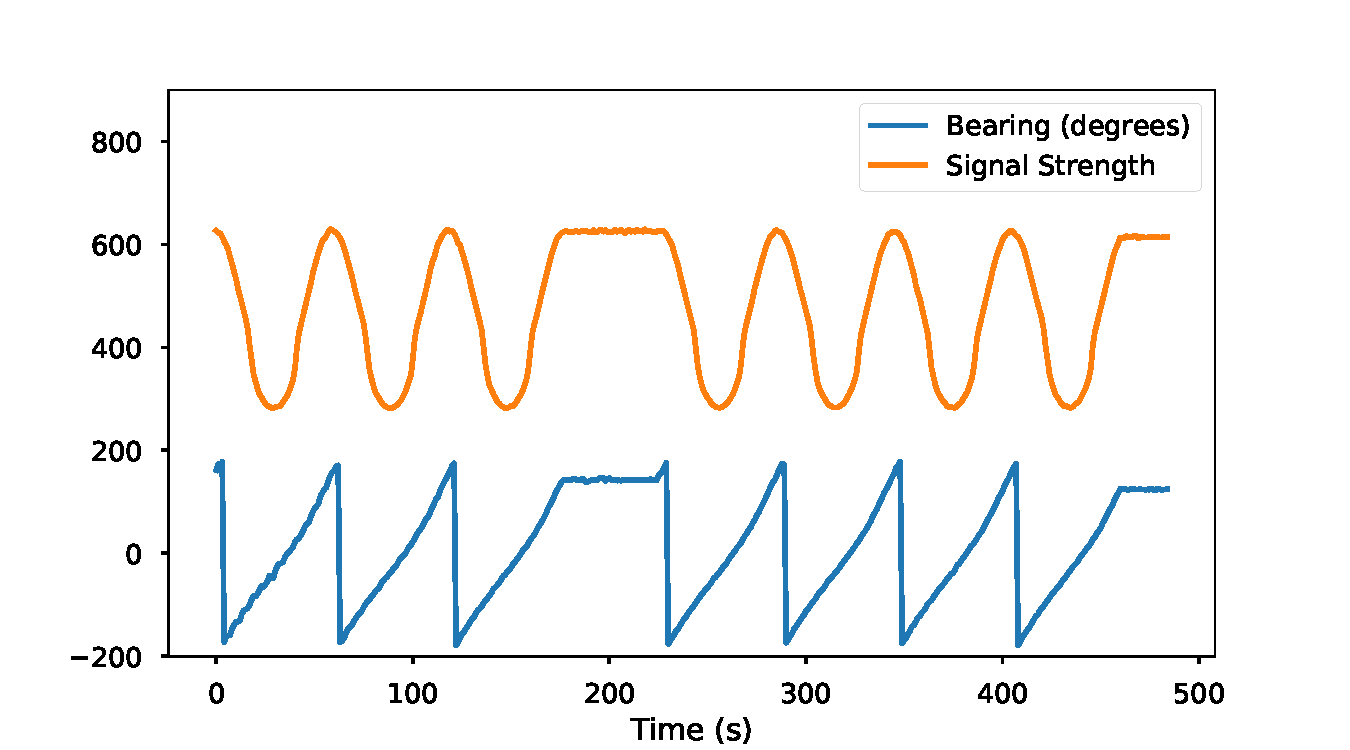
\includegraphics[width=1.0\textwidth]{figures/sample_time_trace.pdf}
\end{figure}


\section{Begin Examples}
And of course, this is just an example of how to do equations.  I'll keep it here as a template for working with equations below.
\begin{align} 
	\begin{split}
	(x+y)^3 	&= (x+y)^2(x+y)\\
					&=(x^2+2xy+y^2)(x+y)\\
					&=(x^3+2x^2y+xy^2) + (x^2y+2xy^2+y^3)\\
					&=x^3+3x^2y+3xy^2+y^3
	\end{split}					
\end{align}

\subsection{Example of a susection}
Subsection text with another equation.  And here is a figure.

\begin{align}
	A = 
	\begin{bmatrix}
	A_{11} & A_{21} \\
  	A_{21} & A_{22}
	\end{bmatrix}
\end{align}
And some more text. And maybe another figure.

\subsubsection{SubSub section}
More text here

\paragraph{Paragraph Header if you want it}
Some stuff in a paragragh.

\paragraph{}
See if this is a new paragraph.


\section{Lists}

\subsection{Example for list (3*itemize)}
\begin{itemize}
	\item First item in a list 
		\begin{itemize}
		\item First item in a list 
			\begin{itemize}
			\item First item in a list 
			\item Second item in a list 
			\end{itemize}
		\item Second item in a list 
		\end{itemize}
	\item Second item in a list 
\end{itemize}

\subsection{Example for list (enumerate)}
\begin{enumerate}
	\item First item in a list 
	\item Second item in a list 
	\item Third item in a list
\end{enumerate}
%%% End document
\end{document}